`% !TeX root = ../defense.tex

\section{Study}
\frame{\sectionpage}


\begin{frame}{Classifiers}
 \begin{itemize}
  \item Used random forests (N=200) to train and test the following models
  \begin{itemize}
    \item baseline 1: current dialog act label.
    \item baseline 2: current and previous dialog acts.
    \item summary model: just the summary features.
    \item full model: summary features and the current and previous dialog acts.
  \end{itemize}
  \item Evaluation was done using 10 fold cross validation.
  \item Run grid search to find the optimal hyper parameters.
  \end{itemize}
\end{frame}{}

\begin{frame}{Result for Random Forest Classifier}
\begin{table}[ht!]
\begin{center}
\begin{tabular}{lrrrrr}
\hline
{}  &  Accuracy &        F1 &  Precision &    Recall &   AUC \\
\hline
baseline 1 &  62.79\% &  57.81\% &   74.98\% &  47.04\% &  65.99\% \\
baseline 2 &  74.89\% &  74.87\% &   81.84\% &  69.00\% &  81.11\% \\
summary    &  65.54\% &  69.32\% &   67.22\% &  71.36\% &  69.46\% \\
full       &  75.75\% &  77.59\% &   77.50\% &  77.83\% &  83.78\% \\
\hline
\end{tabular}
\end{center}
\caption{Precision, recall and F1 results using Random Forests }
\label{table:result}
\end{table}
\end{frame}

\begin{frame}{Result for Gradient Boosting}
\begin{table}[ht!]
\begin{center}
\begin{tabular}{lrrrrr}
\hline
{}  &  Accuracy &        F1 &  Precision &    Recall &   AUC \\
\hline
baseline 1 &  62.79\% &  57.81\% &   74.98\% &  47.04\% &  65.99\% \\
baseline 2 &  74.88\% &  74.82\% &   81.92\% &  68.86\% &  81.10\% \\
summary    &  67.91\% &  71.30\% &   69.20\% &  73.55\% &  72.64\% \\
all        &  76.57\% &  78.74\% &   77.44\% &  80.11\% &  84.84\% \\
\hline
\end{tabular}
\end{center}
\caption{Precision, recall and F1 results using Gradient boost classifier }
\label{table:result2}
\end{table}
\end{frame}


\begin{frame}{ROC curves and AUC of different models}
\begin{figure}
 \centering
 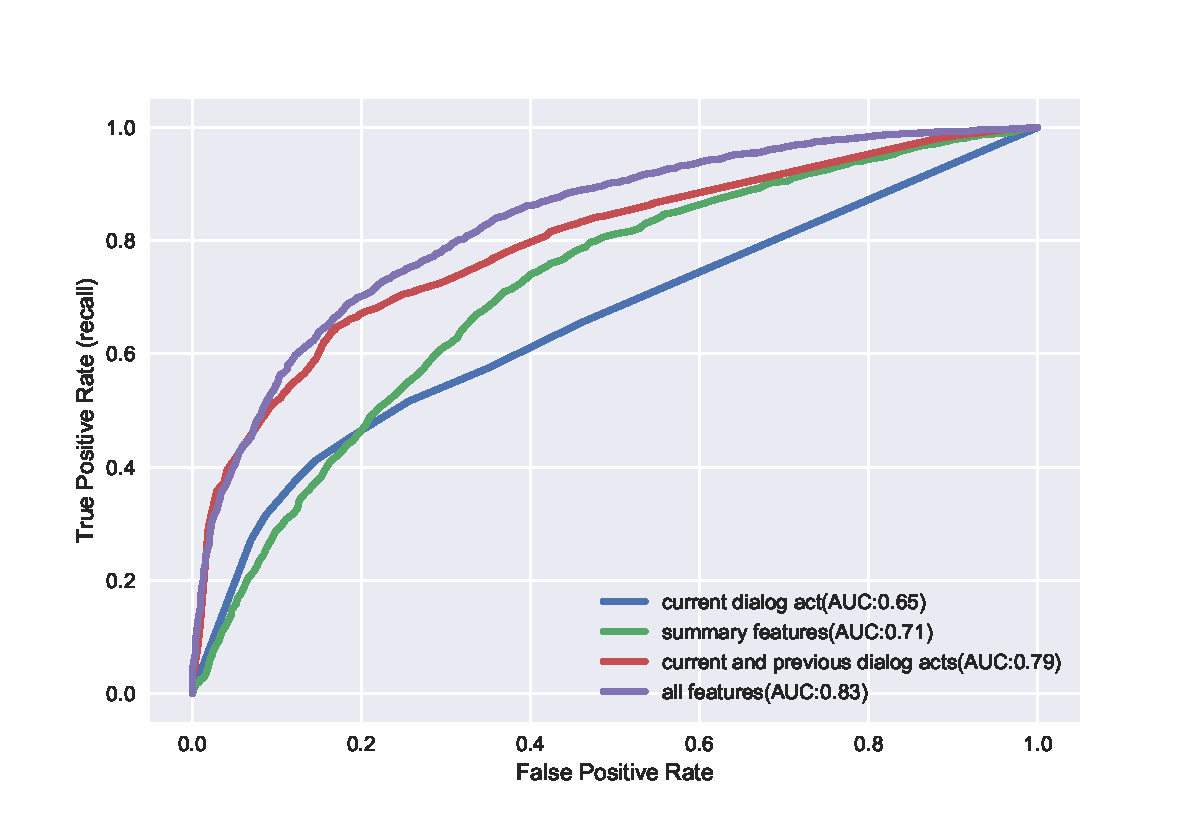
\includegraphics[width=32em]{../scikitlearn/figures/roc.pdf}
 \end{figure}
\end{frame}

\begin{frame} {Sensitivity to Measurement Start Time}
\begin{table}
\begin{center}
\begin{tabular}{lrrrrrrr}
\hline
{} & 0s & 15s & 30s & 45s & 60s & {\bf 120s} & 180s  \\
\hline
baseline 1 & 65.99\% & 66.10\% & 66.12\% & 66.09\%  & 66.02\% & 65.98\% & 66.05\%  \\
baseline 2 & 81.11\% & 81.21\% & 81.24\% & 81.20\%  & 81.15\% & 80.92\% & 80.68\%  \\
summary    & 69.46\% & 69.51\% & 69.43\% & 69.49\%  & 69.57\% & 69.10\% & 69.21\%  \\
full       & 83.78\% & 83.87\% & 83.85\% & 83.80\%  & 83.61\% & 83.19\% & 82.80\%  \\
\hline
\end{tabular}
\end{center}
\caption{ AUC Score in relation to the start of the dialog }
\label{table:starttime}
\end{table}

\end{frame}{}
